\chapter{Decay Heat: The Source That Will Not Switch Off}
\label{ch:decay}

\section{Why decay heat matters for stability and safety}

The point kinetics equations describe the \emph{fission} power, which responds
within seconds to a scram. But roughly $7\%$ of a reactor's steady-state thermal
power comes not from fission directly but from the radioactive decay of fission
products accumulated in the fuel. This \textbf{decay heat} cannot be switched off
by inserting control rods: it is governed by the half-lives of hundreds of
nuclides and decays only with time. Immediately after shutdown from full power,
decay heat is about $6\!-\!7\%$ of the previous power; it falls to roughly $1\%$
after an hour and continues to decline over days. For a $3000\unit{MW}$ thermal
core, $7\%$ is $210\unit{MW}$---a space-heater the size of a small power
station that turns on the instant you shut the reactor down and that must be
removed continuously to prevent the fuel from melting.

Decay heat is the reason a reactor is never truly ``off'' from a thermal
standpoint, and it is the link between a reactivity transient and a thermal
catastrophe: at Chernobyl, at Three Mile Island, and at Fukushima, decay heat
was the persistent source that turned a loss of cooling into core damage. For
stability theory it matters because it sets a floor on the thermal source term
and because, in fast transients, a small additional decay-heat contribution adds
to the energy that feedback must absorb.

\section{The Way--Wigner correlation}

A classic engineering estimate of decay power after an infinitely long
irradiation is the Way--Wigner correlation,
\begin{equation}
\frac{P_d(t)}{P_0} \approx 0.066\left[\,t^{-0.2} - (t+t_0)^{-0.2}\,\right],
\label{eq:waywigner}
\end{equation}
where $t$ is the time since shutdown and $t_0$ the operating time, both in
seconds. For $t_0\to\infty$ this reduces to $P_d/P_0\approx 0.066\,t^{-0.2}$.
Figure~\ref{fig:decay} plots this approximation. The slow, power-law decline---a
consequence of the broad distribution of fission-product half-lives---is the
defining feature: there is no single time constant, and the heat lingers for a
long time.

\begin{figure}[H]
\centering
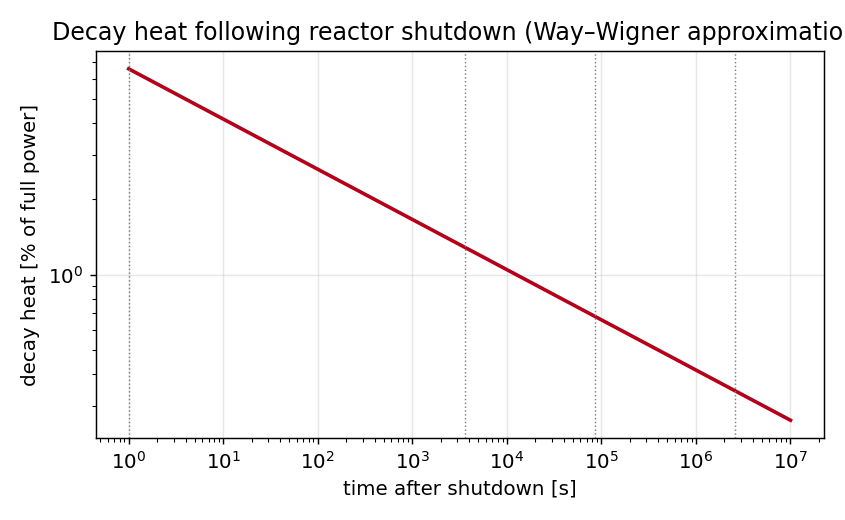
\includegraphics[width=0.74\linewidth]{figures/decay_heat.png}
\caption{Decay heat as a fraction of full power following shutdown, from the
Way--Wigner approximation \eqref{eq:waywigner}. The power-law tail reflects the
broad spectrum of fission-product half-lives; the heat cannot be turned off,
only waited out and removed.}
\label{fig:decay}
\end{figure}

More accurate standards (ANSI/ANS-5.1) sum contributions from the major
fissioning nuclides ($^{235}$U, $^{239}$Pu, $^{238}$U) with tabulated
coefficients, and add the actinide contributions from $^{239}$U and $^{239}$Np,
which are significant in the first day. For our purposes the Way--Wigner picture
captures the essential physics: a large, slowly decaying, irreducible source.

\section{Decay heat in the kinetics model}

Decay heat can be appended to the point kinetics framework with its own set of
decay-heat groups $\omega_k$, in direct analogy with the precursors:
\begin{equation}
P_{\text{total}}(t) = P_f(t) + \sum_k \omega_k(t),\qquad
\frac{\dd \omega_k}{\dd t} = \kappa_k P_f(t) - \lambda_k^{(d)}\omega_k(t),
\end{equation}
where $\kappa_k$ are the energy fractions and $\lambda_k^{(d)}$ the decay-heat
group constants. In a fast power transient the fission term $P_f$ dominates and
decay heat is a small correction; in the aftermath of a scram it is the only term
left. The companion software of Chapter~\ref{ch:comp} includes decay-heat groups
for exactly this reason.

\section{The thermal consequence: a worked estimate}

\begin{example}[Adiabatic heat-up after loss of cooling]
Suppose cooling is lost just after shutdown from full power $P_0$, and decay heat
is initially $q=0.06\,P_0$. If the core thermal mass is $C$ and no heat is
removed, the fuel temperature rises at
\begin{equation}
\frac{\dd \Tf}{\dd t} = \frac{q}{C}.
\end{equation}
For a core with $C\sim 10^{7}\unit{J/K}$ and $P_0=3\times10^{9}\unit{W}$, the
initial decay power is $q\approx 1.8\times10^{8}\unit{W}$, so
$\dd\Tf/\dd t\approx 18\unit{K/s}$. Starting near the normal operating
temperature, the fuel would reach the melting point of $\mathrm{UO_2}$
($\sim 2800\degC$) in a few minutes. This is the quantitative basis for the
absolute requirement of emergency core cooling, and it explains why the
\emph{thermal} accident can proceed even after the \emph{nuclear} reaction is
stopped.
\end{example}

\keypoint{Stopping fission is necessary but not sufficient for safety. Decay heat
is an irreducible thermal source of several per cent of full power that must be
removed for days. Thermal stability concerns the fission transient; thermal
\emph{safety} also demands that the decay-heat path to the ultimate heat sink is
never lost. Chernobyl began as a fission-power instability; its enduring danger
came from the decay heat in the wrecked core.}

\section{Summary of Part I}

We now have the foundations. Reactivity \eqref{eq:reactivity} measures distance
from criticality; the six-factor formula \eqref{eq:sixfactor} localises where
feedback acts; the point kinetics equations \eqref{eq:prk} give the dynamics,
with delayed neutrons setting the controllable timescale and the inhour equation
\eqref{eq:inhour} the period; the prompt-jump \eqref{eq:promptjump} captures the
instantaneous response; and decay heat provides an irreducible thermal source.
Part~II turns to the thermal side: how the fission power becomes temperature, and
how temperature, in turn, becomes reactivity---closing the feedback loop whose
sign decides stability.


\section*{Exercises}
\addcontentsline{toc}{section}{Exercises}
\begin{enumerate}[leftmargin=*,itemsep=2pt]
\item Using the Way--Wigner approximation, estimate the decay-heat fraction at $1\,$s, $1\,$h, and $1\,$day after shutdown.
\item For a $3000\,$MW$_\text{th}$ core with thermal mass $C=10^7\,$J/K and $6\%$ initial decay heat, estimate the adiabatic heat-up rate just after a loss of cooling.
\item Why does decay heat decline as a power law rather than a single exponential?
\item Explain why stopping the fission chain reaction does not remove the need for cooling.
\item How does decay heat connect a reactivity transient to a thermal accident?
\end{enumerate}
